\documentclass[letterpaper,12pt]{article}
\usepackage{lipsum}  
\usepackage{graphicx}
\usepackage{subcaption}
\usepackage[english]{babel}
\usepackage{fancyhdr}

\graphicspath {{figures/}}

\setlength{\headheight}{15pt}

\pagestyle{fancy}
\fancyhf{}
\lhead{\textbf{Version:} 1  \textbf{Revision:} \today}
\rhead{\thepage}
\lfoot{Cole Kampa}
\rfoot{\textit{Mu2e: University of Minnesota}}

\renewcommand{\footrulewidth}{1pt}


\begin{document}
\begin{titlepage}
	\centering
	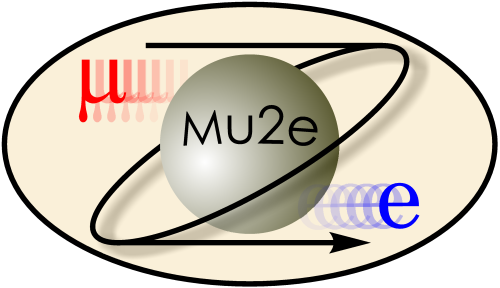
\includegraphics[width=0.5\textwidth]{mu2e_logo_oval.png}\par\vspace{2cm}
	{\scshape\LARGE Automated Sense Wire Tensioner: \\ Project Status Update 1\par}
	\vspace{3cm}
	{\Large Cole Kampa\par}
	%\vspace{3cm}
	\vspace{3.5cm}
	{\large University of Minnesota\par}
 	\vspace{.5cm}
	{\large \today \par}
	% Bottom of the page
	\vfill
	{kampa041@umn.edu\par}
\end{titlepage}

\clearpage
\setcounter{page}{2}


\section*{Status \& Milestones}
\begin{itemize}{
\item{
Proof of concept complete.
}
\item{
Operational code to tension to $(80.0\pm 0.5)\ gf$ (limited by spring strength)
}
\item{
\textbf{Speed:}
}
\item{
\textbf{Cost Estimate:}
}
}
\end{itemize}
Use as many or few of these sections as you see fit.
%%Insert your text here...same follows below%%

\section*{Advantages}
We compare to the current method of using a system of pulleys and a hanging mass.
\begin{itemize}{
\item{

}
\item{

}
\item{

}
}
\end{itemize}

\section*{Potential Advantages}




\section*{Current Problems}

\section*{Images}
\begin{figure} [h]
		\centering
		
\includegraphics[width=0.25\textwidth]{dummy.png}
		\caption{Dummy figure.}
		\label{fig:dummy}
\end{figure}


\end{document}